% -****- reftex-default-bibliography:
% ("/home/mkramer/physics/thesis/biblio.bib") -*-
\documentclass[../thesis.tex]{subfiles}

\begin{document}

\chapter{Calibration}
\label{chap:calib}

\begin{comment}
  Add channel quality to this chapter!
\end{comment}

\section{Overview}

For the antineutrino detectors \cite{SideBySide} and water pools, the Daya Bay
\cite{An_2017} DAQ system outputs little more than timestamped PMT hits, grouped
into readout windows and tagged with trigger information. These hits take the
form of ADC readings from the peak-finding electronics, along with the TDC count
at the time that each (shaped) PMT waveform crossed the disciminator's
threshold. In order to carry out any sort of physics analysis, it is necessary
to first convert this raw ADC and TDC data into the higher-level quantities of
photoelectron count and photon arrival time, and then to combine individual
channels into event parameters such as energy and position.

This chapter describes the first half of that process; namely, the detector
calibration and data processing involved in the channel-by-channel calculation
of hit time and charge. These calibrated quantities are fundamental in that they
are used in all further analysis stages and by all reconstruction
algorithms. Accuracy is vital, as any bias in the channel charge will be
reflected in the total event energy and in any (charge-based) vertex
reconstruction; likewise, accurate times are important for time-based vertex
reconstructions. Furthermore, it is necessary to identify and exclude any
misbehaving channels, a process that will also be discussed here.

\section{Timing calibration}

The timing calibration takes each hit's TDC count\footnote{I.e., the number of
  ticks that elapsed between the hit and the trigger} and converts it into an
estimate of the time at which the photon struck the photocathode. The absolute
time is unimportant, but for the purpose of time-based vertex (or track)
reconstruction, the \emph{relative} times between channels must be accurately
determined. These calibrated times, in addition to their use in vertex
reconstruction, are also used in defining the time window for hit selection
(performed during the \emph{event's} charge calculation, described in the next
chapter).\footnote{To be fair, given that this window is 400~ns wide, and the
  timewalk correction is on the order of a few~ns, the raw times would actually
  suffice for hit selection.}

This process involves subtracting out a channel-specific offset (corresponding
to cable length, etc.) with an additional correction for the charge-dependent
\emph{timewalk effect}, in which smaller pulses take longer than larger ones to
cross the discriminator's threshold. The offset, as well as a parameterization
of the timewalk curve, is stored in the calibration database and applied to the
TDC readings during data processing. We now discuss the preparation of these
calibration constants.

\subsection{Calibration constant preparation}

To measure each channel's offset and timewalk profile, we require a well-defined
event vertex and an external source of $T_0$ (true event time)
information.\footnote{There is a natural variance in the timing of readout
  triggers, smearing the TDC measurements between different events. Knowledge of
  $T_0$ effectively provides knowledge of the trigger ``jitter'' for each event,
  allowing it to be subtracted out. Without this information, it is impossible
  to obtain a useful timewalk curve.} Toward that end, Daya Bay uses LED
calibration runs in which the LED is positioned at the center of the
detector. When a pulse is sent to the LED, a ``hit'' is also sent to the FEE
from a ``fake'' $T_0$ channel. For each PMT hit on channel $i$, we take its TDC
count $N$ and calculate a corrected time
\[ t = \frac{N_0 - N}{f_\mathrm{TDC}} - \frac{n r_i}{c}, \] where $N_0$ is the
TDC count of the $T_0$ channel, $f_\mathrm{TDC}$ is the TDC frequency, and
$nr_i/c$ gives the time of flight to channel $i$. The t.o.f. subtraction ensures
that we can directly compare channels from different rings without any further
geometric considerations.

In the next step, a 2D histogram is constructed for each channel by taking all
of the channel's hits (within a reasonable time window) across all events, and
plotting each hit's corrected time $t$ against its ADC count $q$. This
histogram's profile is then fit to the six-parameter functional form
\[ t(q) = a_1 + a_2 \exp (-a_3 q) + a_4 \exp (-a_5 q) + a_6 \log q, \] which was
empirically found to produce good fits under appropriate restrictions on the
parameters. \autoref{fig:timewalk}~ shows an example of a timewalk fit.

After a manual verification of fit quality, the six parameters for each channel
are uploaded to the database and marked with a suitable validity
period. Whenever the electronics have been modified in a way that could affect
the timing (such as a cabling change or board replacement), a new set of
constants is prepared for the affected AD, using this same procedure.

% Because $t(q)$ gives the \emph{time since trigger}, which is on the order of a
% microsecond, a single global $\mu$s-scale offset (the average of all the
% $a_1$'s, to be precise) is subtracted from each $a_1$. This ensures that when
% we later use $t(q)$ as a \emph{correction}, we don't apply a large offset to
% the times we are correcting.

\begin{figure}
  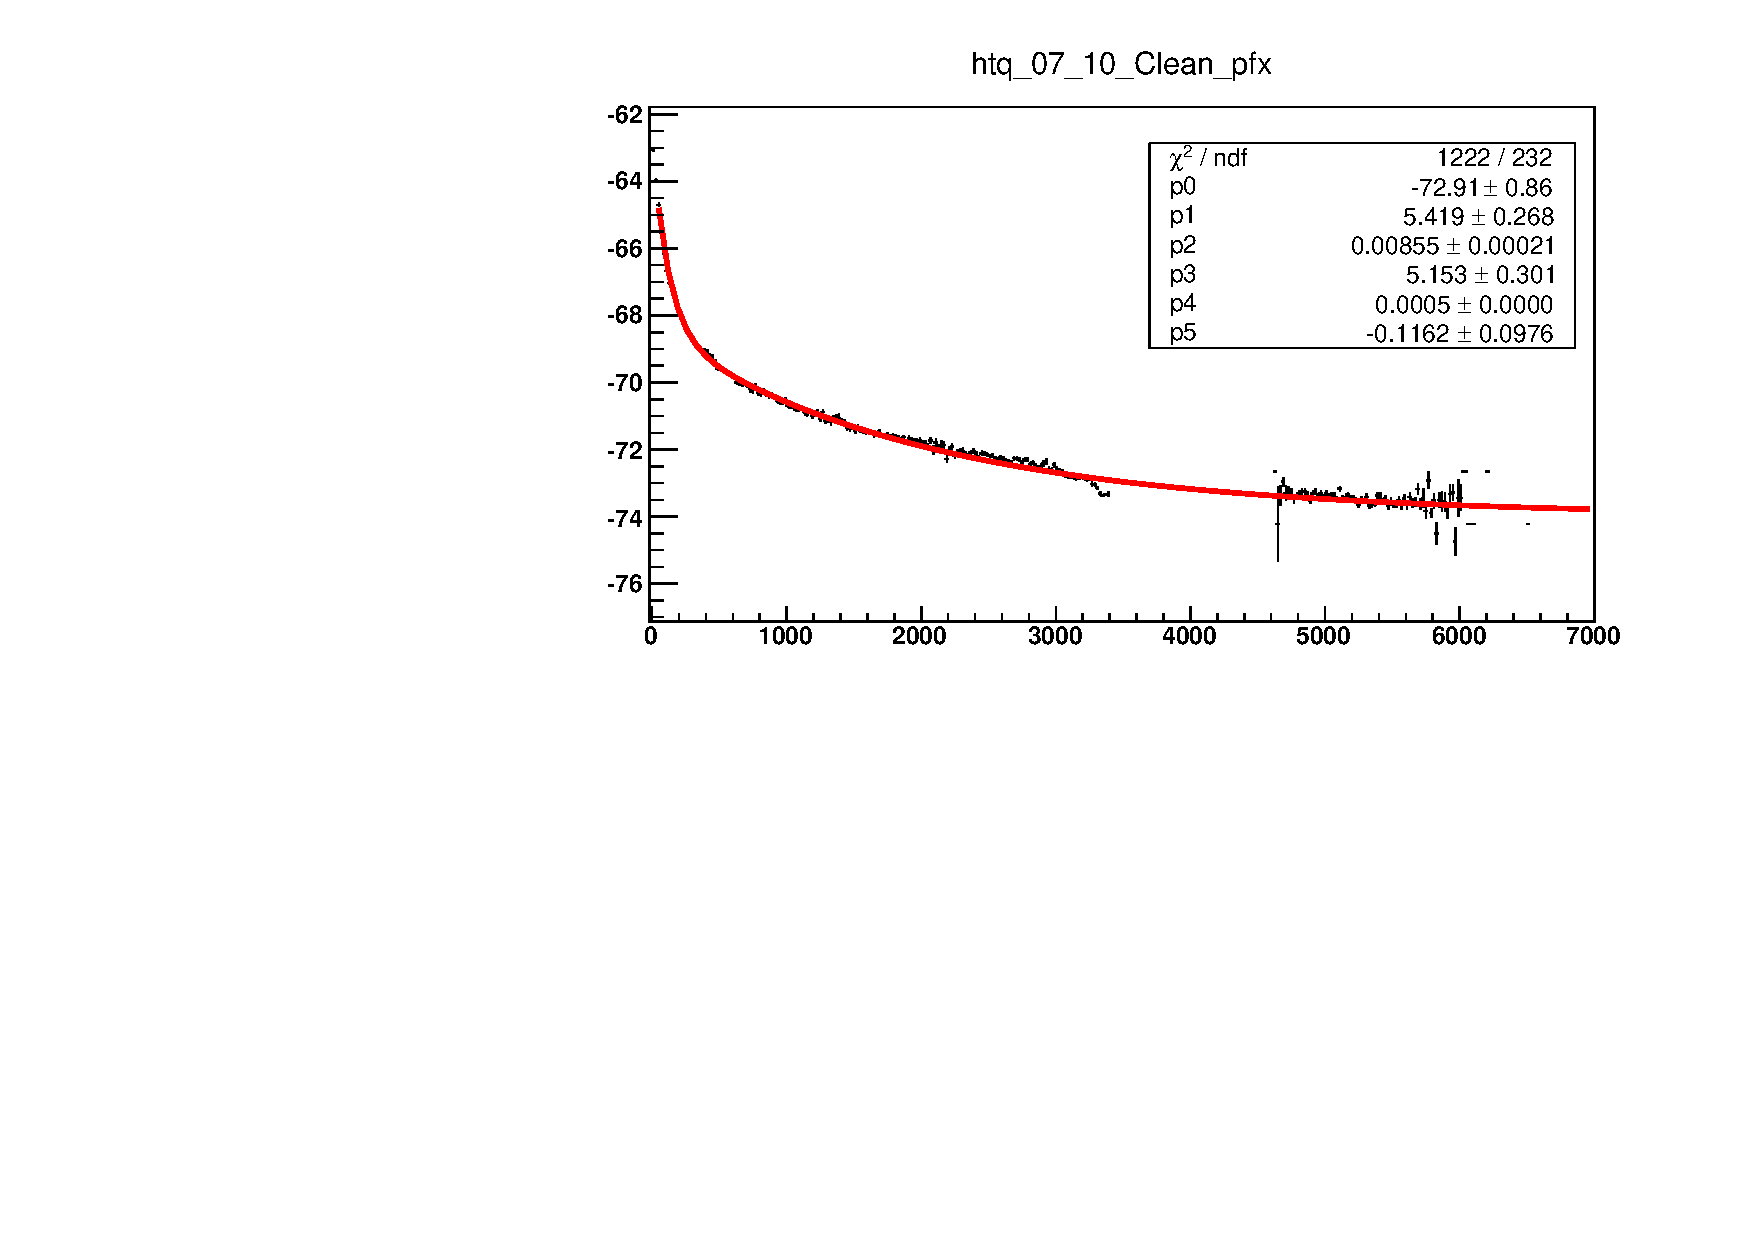
\includegraphics[scale=0.7]{fit_eh1_ad1_r7c10.pdf}
  \caption{An example of a timewalk fit.}
  \label{fig:timewalk}
\end{figure}

\begin{comment}
  Show the tof-corrected times; comment on TDC discretization.
\end{comment}

\subsection{Calculation of corrected times}

Once the calibration parameters are in the database, applying them to the raw
data is straightforward. For each hit, we take the ADC count $q$ and plug it
into the function $t(q)$, with the parameters taken from the database. Then,
using the channel's raw TDC count $N$, the calibrated time $t_c$ is calculated
as
\[ t_c = -\frac{N}{f_\mathrm{TDC}} - t(q), \] After this is done, we have a
calibrated time, in ns, for each hit, which can be directly and accurately
compared to other hits in other channels, regardless of how much charge each
channel saw and regardless of intrinsic variations between channels. This meets
the requirements for time-based vertex and track reconstruction.

\section{Gain calibration}

At a given operating voltage, every PMT will produce a unique amount of charge
per photoelectron, even among other PMTs of the same model. Furthermore, this
response tends to vary with time and environmental conditions, demanding a
periodic recalibration of the gain. In Daya Bay, the HV for each channel was
initially fixed in order to provide a nominal gain of $1 \times 10^7 \pm
5\%$. During the gain calibration, the true gain is measured and stored in the
database. This is expressed as the number of ADC counts (i.e., the FEE's charge
measurement) per photoelectron.

To measure the gain, Daya Bay uses ``dark noise'', the thermal emission of
electrons from the photocathode\footnote{Each dynode can of course also emit
  electrons, but the collected charge is attenuated by $\mathcal{O}(5^n)$ for
  emission from the $n$th dynode. This effect can therefore be safely neglected
  for our purposes.}. Due to the $\sim\mu$s width of the readout window, it is
possible to collect dark noise by looking for isolated hits in the few hundred
ns preceding each detector-wide trigger. This can be done using ordinary physics
data, eliminating the need for special gain calibration runs\footnote{In the
  past, Daya Bay has in fact employed a separate, redundant gain calibration
  using LED runs, which gave results consistent with this ``rolling gain''
  method.}. In order to acquire enough statistics, roughly six hours of data are
needed, limiting the frequency of calibration updates to 4 per day. Fortunately,
this is far shorter than the timescale of gain variations; most channels drift
by no more than a few percent per year. % CHECKME, add stability plot

Thermal emission is a Poisson process, and the collected charge per primary
electron is normally distributed. Convolving the two gives a model of the charge
distribution for dark noise hits,
\[ P(Q) = \sum_{n^=1}^{\infty} \frac{\mu^n e^{-\mu}}{n!}
  \frac{1}{\sigma_{\mathrm{SPE}}\sqrt{2n\pi}} \exp\left(-\frac{(Q - n\overline
      Q^{\mathrm{SPE}})^2}{2n\sigma_{\mathrm{SPE}}^2}\right) \] where $\mu$ is
the mean number of photoelectrons, $\overline Q^{\mathrm{SPE}}$ is the average
charge per p.e., and $\sigma_{\mathrm{SPE}}$ is the corresponding spread. Due to
the extremely low probability of observing multiple thermal electrons in a
single hit, the sum was restricted to $n \le 2$ in practice.

Using this model, the dark noise ADC distribution\footnote{The fit is restricted
  to ADC values above 10, as noise in the low-ADC region was found to impair the
  stability of the fit} can be fit for each channel, yielding the channel's
characteristic values of $\mu$, $\overline Q^{\mathrm{SPE}}$, and
$\sigma_{\mathrm{SPE}}$. In particular, $\overline Q^{\mathrm{SPE}}$ corresponds
to the channel's gain. These parameters are stored in the database and used
during data processing to calculate the calibrated charge for each channel,
providing the basis of the energy reconstruction, described in the next chapter.

\section{Channel quality}

In order to prevent any biases from being introduced by misbehaving channels, a
channel quality database is consulted during data production, and any tagged
channels are excluded from the total event charge (see next chapter). Bad
channels are identified and tagged during the regular ``keep-up'' processing of
each new data file. Four quantities are used for each data file:

\begin{enumerate}
\item Channel occupancy, i.e., the percentage of events in which the channel
  recorded at least one hit (must be within range);
\item HV average (must be above minimum);
\item HV RMS (must be below maximum);
\item Average baseline-subtracted ADC count (must be within range).
\end{enumerate}

Physics and calibration runs use distinct, empirically tuned cuts on these four
values. If a channel fails any of these cuts, it is marked bad for the duration
of the file's runtime. In most cases, bad channels have been found to result
from HV instability. Fortunately, this has generally been an isolated issue; on
average, there have been around a half-dozen bad channels at any given time,
usually with no more than one per AD.

\subfilebackmatter
\end{document}
